\documentclass{standalone}
\usepackage{textcomp}
\usepackage{pgfplots}
\begin{document}
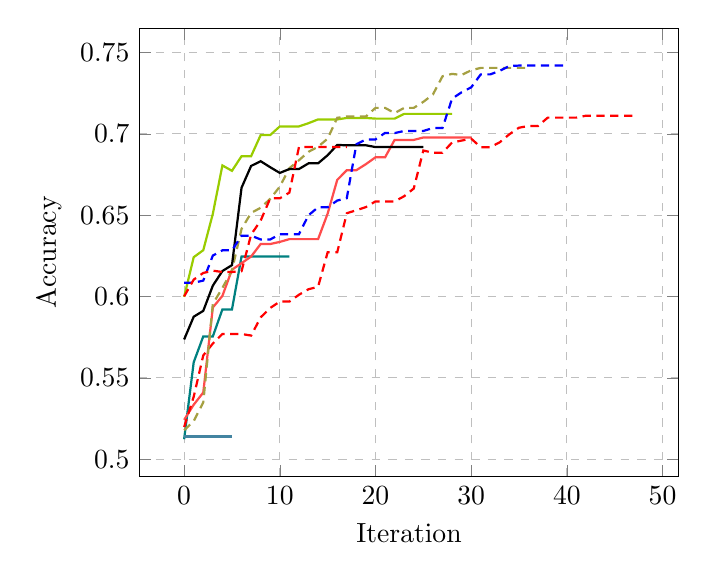
\begin{tikzpicture}
\begin{axis}[
    %title={Training},
    %width=0.8\textwidth,
    %height=0.5\textwidth,
    xlabel={Iteration},
    ylabel={Accuracy},
    %xmin=1, xmax=17,
    %ymin=0.44, ymax=1.1,
    %xtick={2,1024,2048,4096},
    %ytick={0.5,0.6,0.7,0.8,0.9,1.00},
    legend pos=south east,
    ymajorgrids=true,
    xmajorgrids=true,
    grid style=dashed,
    %xmode=log,
    %log ticks with fixed point,
    cycle list name = exotic,
    %cycle list = {
        %{black, mark=square, solid},
        %{red, mark=*, dotted},
        %{green, mark=x, dashed},
        %{blue, mark=+, dash dot},
        %{cyan, mark=o, dash dot dot},
        %{magenta, mark=asterisk, densely dotted},
        %{orange, mark=oplus, densely dashed},
        %{gray, mark=triangle, densely dash dot},
        %{lightgray, mark=diamnond, densely dash dot dot},
        %{brown, mark=star, loosely dotted},
    %}
]

%\begin{scope}[thick, mark options={scale=1.5, solid}]
\begin{scope}[thick, mark=none]
\addplot coordinates{
(0,0.5123)
(1,0.5596)
(2,0.5755)
(3,0.5755)
(4,0.5921)
(5,0.5921)
(6,0.6246)
(7,0.6246)
(8,0.6246)
(9,0.6246)
(10,0.6246)
(11,0.6246)
};
\addplot coordinates{
(0,0.5139)
(1,0.5139)
(2,0.5139)
(3,0.5139)
(4,0.5139)
(5,0.5139)
};
\addplot coordinates{
(0,0.5139)
(1,0.5139)
(2,0.5139)
(3,0.5139)
(4,0.5139)
(5,0.5139)
};
\addplot coordinates{
(0,0.5242)
(1,0.5335)
(2,0.541)
(3,0.5933)
(4,0.6004)
(5,0.6165)
(6,0.6205)
(7,0.6246)
(8,0.6323)
(9,0.6323)
(10,0.6336)
(11,0.6353)
(12,0.6353)
(13,0.6353)
(14,0.6353)
(15,0.651)
(16,0.6717)
(17,0.6777)
(18,0.6777)
(19,0.6814)
(20,0.6856)
(21,0.6856)
(22,0.6963)
(23,0.6963)
(24,0.6963)
(25,0.6978)
(26,0.6978)
(27,0.6978)
(28,0.6978)
(29,0.6978)
(30,0.6978)
};
\addplot coordinates{
(0,0.5998)
(1,0.6242)
(2,0.6285)
(3,0.6509)
(4,0.6806)
(5,0.6773)
(6,0.6863)
(7,0.6863)
(8,0.6993)
(9,0.6993)
(10,0.7046)
(11,0.7046)
(12,0.7046)
(13,0.7066)
(14,0.7089)
(15,0.7089)
(16,0.7089)
(17,0.7098)
(18,0.7098)
(19,0.7098)
(20,0.7094)
(21,0.7094)
(22,0.7094)
(23,0.7123)
(24,0.7123)
(25,0.7123)
(26,0.7123)
(27,0.7123)
(28,0.7123)
};
\addplot coordinates{
(0,0.5198)
(1,0.5384)
(2,0.5638)
(3,0.5711)
(4,0.577)
(5,0.577)
(6,0.577)
(7,0.576)
(8,0.5872)
(9,0.593)
(10,0.5969)
(11,0.5969)
(12,0.6011)
(13,0.6045)
(14,0.606)
(15,0.6272)
(16,0.6272)
(17,0.6512)
(18,0.6531)
(19,0.655)
(20,0.6585)
(21,0.6585)
(22,0.6585)
(23,0.6617)
(24,0.6664)
(25,0.6898)
(26,0.6884)
(27,0.6884)
(28,0.6947)
(29,0.6959)
(30,0.6971)
(31,0.6918)
(32,0.6918)
(33,0.6949)
(34,0.6998)
(35,0.7038)
(36,0.7049)
(37,0.7049)
(38,0.71)
(39,0.71)
(40,0.71)
(41,0.71)
(42,0.7112)
(43,0.7112)
(44,0.7112)
(45,0.7112)
(46,0.7112)
(47,0.7112)
};
\addplot coordinates{
(0,0.5178)
(1,0.5234)
(2,0.5349)
(3,0.5955)
(4,0.6053)
(5,0.6161)
(6,0.6416)
(7,0.6514)
(8,0.6546)
(9,0.6601)
(10,0.6676)
(11,0.6789)
(12,0.6838)
(13,0.689)
(14,0.6921)
(15,0.6971)
(16,0.7099)
(17,0.7107)
(18,0.7107)
(19,0.7107)
(20,0.716)
(21,0.716)
(22,0.7128)
(23,0.716)
(24,0.716)
(25,0.7197)
(26,0.7242)
(27,0.7354)
(28,0.7369)
(29,0.7362)
(30,0.7391)
(31,0.7406)
(32,0.7406)
(33,0.7406)
(34,0.7406)
(35,0.7406)
(36,0.7406)
};
\addplot coordinates{
(0,0.5736)
(1,0.5876)
(2,0.5912)
(3,0.6067)
(4,0.6157)
(5,0.6193)
(6,0.6669)
(7,0.6803)
(8,0.6832)
(9,0.6795)
(10,0.676)
(11,0.6784)
(12,0.6784)
(13,0.6819)
(14,0.6819)
(15,0.6869)
(16,0.6932)
(17,0.693)
(18,0.693)
(19,0.693)
(20,0.6919)
(21,0.6919)
(22,0.6919)
(23,0.6919)
(24,0.6919)
(25,0.6919)
};
\addplot coordinates{
(0,0.6085)
(1,0.6085)
(2,0.6098)
(3,0.6252)
(4,0.6284)
(5,0.6284)
(6,0.6374)
(7,0.6374)
(8,0.6351)
(9,0.6351)
(10,0.6383)
(11,0.6383)
(12,0.6383)
(13,0.65)
(14,0.6549)
(15,0.6549)
(16,0.659)
(17,0.6605)
(18,0.6936)
(19,0.6966)
(20,0.6966)
(21,0.7006)
(22,0.7005)
(23,0.7018)
(24,0.7018)
(25,0.7018)
(26,0.7036)
(27,0.7036)
(28,0.7216)
(29,0.7256)
(30,0.7286)
(31,0.7366)
(32,0.7366)
(33,0.7388)
(34,0.7418)
(35,0.742)
(36,0.742)
(37,0.742)
(38,0.742)
(39,0.742)
(40,0.742)
};
\addplot coordinates{
(0,0.6001)
(1,0.6104)
(2,0.6145)
(3,0.6159)
(4,0.6151)
(5,0.6151)
(6,0.6156)
(7,0.6381)
(8,0.6467)
(9,0.6604)
(10,0.6604)
(11,0.6639)
(12,0.6919)
(13,0.6919)
(14,0.6919)
(15,0.6919)
(16,0.6919)
(17,0.6919)
};
\end{scope}

\end{axis}
\end{tikzpicture}
\end{document}
